\documentclass[modern]{aastex62}

\usepackage{graphicx}
\usepackage{xcolor}
\usepackage{xspace}
\usepackage[sort&compress]{natbib}
\usepackage[hang,flushmargin]{footmisc}


% style tweaks
\newcommand{\acronym}[1]{{\small{#1}}}
\newcommand{\project}[1]{\textsl{#1}}
\newcommand{\code}[1]{{\texttt{#1}}}
\newcommand{\todo}[1]{\textcolor{red}{#1}}

% the following is stolen from Adrian Price-Whelan (github.com/adrn/latex-init):
\usepackage{hyperref}
\definecolor{niceblue}{rgb}{0.0, 0.4, 0.65}
\definecolor{linkcolor}{rgb}{0.02,0.35,0.55}
\definecolor{citecolor}{rgb}{0.4,0.4,0.4}
\hypersetup{colorlinks=true,linkcolor=linkcolor,citecolor=citecolor,
            filecolor=linkcolor,urlcolor=linkcolor}
\hypersetup{pageanchor=false}

% astronomy
\newcommand{\teff}{\ensuremath{T_{\rm eff}}}
\newcommand{\logg}{\ensuremath{\log g}}
\newcommand{\feh}{\ensuremath{\mathrm{[Fe/H]}}}
\newcommand{\vt}{\ensuremath{v_t}}
\newcommand{\mh}{\ensuremath{\mathrm{[M/H]}}}
\newcommand{\xh}{\ensuremath{\mathrm{[X/H]}}}
\newcommand{\I}{\textsc{I}}
\newcommand{\II}{\textsc{II}}
\newcommand{\vsini}{\ensuremath{v \sin{i}}}
\newcommand{\gcm}{\ensuremath{\mathrm{g}~\mathrm{cm}^{-3}}}
\newcommand{\kms}{\ensuremath{\mathrm{km}~\mathrm{s}^{-1}}}
\newcommand{\masyr}{\ensuremath{\mathrm{mas}~\mathrm{yr}^{-1}}}
\newcommand{\msun}{\ensuremath{\mathrm{M}_\odot}}
\newcommand{\ang}{\text{\normalfont\AA}}


\newcommand{\TF}{\code{TensorFlow}\xspace}
\newcommand{\python}{\code{python}\xspace}
\newcommand{\HARPS}{\project{\acronym{HARPS}}\xspace}
\newcommand{\HIRES}{\project{\acronym{HIRES}}\xspace}
\newcommand{\RV}{\acronym{RV}\xspace}
\newcommand{\RVs}{\acronym{RV}s\xspace}


% stolen from Ben Pope:
\newcommand{\kepler}{\emph{Kepler}\xspace}
\newcommand{\hipparcos}{\emph{Hipparcos}\xspace}
\newcommand{\gaia}{\emph{Gaia}\xspace}
\newcommand{\ktwo}{\emph{K2}\xspace}
\newcommand{\TESS}{\emph{\acronym{TESS}}\xspace}

% misc shortcuts
\newcommand{\flatiron}{Flatiron Institute, Simons Foundation, 162 Fifth Ave, New York, NY 10010, USA}
\newcommand{\chicago}{Department of Astronomy and Astrophysics, University of
Chicago, 5640 S. Ellis Ave, Chicago, IL 60637, USA}
\newcommand{\USP}{Universidade de Sao Paulo}
\newcommand{\MIT}{MIT}

\graphicspath{ {./figures/} }
\newcommand{\hoststar}{\acronym{HIP}\ 96160\xspace}
\newcommand{\plname}{\acronym{HIP}\ 96160b\xspace}
\newcommand{\plmass}{$13.1 \pm 5.0\ \mearth$\xspace}
\newcommand{\plradius}{$3.41 \pm 0.01\ \rearth$\xspace}
\newcommand{\pldensity}{\todo{TODO} \gcm\xspace}
\newcommand{\stmass}{$1.0 \pm x\ \msun$\xspace}
\newcommand{\stradius}{$1.0 \pm x\ \rsun$\xspace}

\shorttitle{Warm Sub-Neptune Transiting a Solar Twin}
\shortauthors{Bedell et al.}

\setlength{\parindent}{1.4em} % trust in Hogg
\begin{document}\sloppy\sloppypar\raggedbottom\frenchspacing % trust in Hogg

\graphicspath{ {figures/} }
\DeclareGraphicsExtensions{.pdf,.eps,.png}

\title{A Warm Sub-Neptune Transiting a Solar Twin in TESS}

\author[0000-0001-9907-7742]{Megan Bedell}
\affiliation{\flatiron}

\author{Dan Foreman-Mackey}
\affiliation{\flatiron}

\author{Jorge Melendez}
\affiliation{\USP}

\author{Lorenzo Spina}
\affiliation{Monash}

\author{Chelsea Huang}
\affiliation{\MIT}

\author{Jennifer Burt}
\affiliation{\MIT}

\author{Jhon Yana Galarza}
\affiliation{\USP}

%\author{Jacob L. Bean}
%\affiliation{\chicago}


\author{\todo{other STPS folks}}



\correspondingauthor{Megan Bedell}
\email{mbedell@flatironinstitute.org}


\begin{abstract}\noindent
We present the discovery of \plname, a sub-Neptune planet transiting a nearby solar twin star. 
The host star has been observed extensively as part of a radial velocity (\RV) campaign targeting solar twins with \HARPS. 
From these data, we find a planetary minimum mass of \plmass. 
We also measure a radius of \plradius from \TESS photometry. 
Taken together, the resulting planetary bulk density of \pldensity implies that an extended atmosphere is present, making this system an excellent candidate for transmission spectroscopic follow-up. 
The extreme similarity between \hoststar and the Sun means that both the absolute planetary mass and radius and the bulk composition of the \hoststar system can be measured with unusually high accuracy. 
We discuss the role of this system as a benchmark comparison to our own Solar System.

%\todo{We use the composition of the host star to place constraints on the planet's potential properties and show that it is likely to be... ??}

% Precise characterization of exoplanet host stars is critical to our understanding of their properties. 
% However, stellar spectroscopic characterization can be plagued with 
\end{abstract}


\section{Introduction}
\label{s:intro}

The thousands of diverse exoplanets discovered by transit search missions like \TESS and \kepler are hosted by a similarly diverse set of stars. 
Some of the best-known exoplanets orbit M dwarf host stars, including Trappist-1 \citep{} and GJ~1214 \citep{}. 
These systems are an exciting opportunity because the transit signal of a habitable-zone terrestrial planet around an M dwarf is relatively easy to detect and may be followed up with transmission spectroscopy to probe the planet's atmosphere. 
On the other hand, detailed constraints on the properties of the host star are limited in precision for M dwarfs. 
Asteroseismically oscillating stars, evolved giants, eclipsing binaries, and other more exotic host stars can fill in some of these gaps, setting very accurate planet radii for their systems through precisely measured host star properties. 
Finally, Sun-like stars (here defined as FGK main-sequence stars) make up a significant fraction of known planet hosts \todo{(give numbers)}. 
These systems can be seen as an intriguing glimpse of alternate paths our own Solar system might have taken in its early formation, and they represent our best opportunity to discover a ``truly Earth-like'' exoplanet that exists under conditions as similar as possible to our own planet.

Solar twins are an important subset of Sun-like stars. 
Typically defined by their extreme similarity to the Sun in fundamental spectroscopic properties (\teff\ within 100 K, \logg\ within 0.1 dex, and \feh\ within 0.1 dex of Solar values), these stars must by definition have such similar photospheric conditions to the Sun that their spectra can be directly compared. 
The result of this line-by-line differential spectroscopic analysis is uniquely precise abundance measurements for the star and thereby for the star-planet system \citep[see e.g.][who achieve 0.01 dex or 2\% precision on abundance measurements for over 30 elements]{Bedell18, Spina18}. 
Similarly precise measurements may be made of the star's age, mass, radius, and other fundamental properties by combining isochronal models with the spectroscopic measurements \citep{}. 
It is worth emphasizing that these properties are measured with extreme precision (not necessarily accuracy) relative to the Sun, our most thoroughly characterized planet host. 
Planetary systems around solar twin stars are therefore useful both as individual well-characterized planets but also as a prime sample for comparative studies delving into any subtle differences between stars that host planets of different types.

Unfortunately, the sample of known planets around solar twins is very limited in number at present. 
\todo{(give a rundown)}

%The Transiting Exoplanet Survey Satellite (\TESS) has detected over one thousand candidate exoplanets to date. 
%The majority of these newly discovered planets orbit bright, nearby stars, making them perfectly suited for follow-up observations, including mass measurements and atmospheric spectroscopy. 
%Unlike most \kepler systems, then, observational signal-to-noise may not be the dominant term in the error budget for the planet masses and other properties measured by ground-based follow-up campaigns.


In this work, we present the first planet detected by \TESS to orbit a solar twin star. 
\object[HIP96160]{\hoststar} is a \stmass, \stradius G2V star with a spectrum nearly identical to that of the Sun. 
Previous studies have derived stellar properties and photospheric abundances for this \hoststar that are accurate to the $1\text{--}2\%$ level.

\hoststar has been studied extensively through a dedicated \RV planet search and spectroscopic abundance survey targeting solar twin stars with the High Accuracy Radial velocity Planet Searcher spectrograph \citep[\HARPS][]{mayor03}. 
Its planet, however, was not confidently detected until \TESS transits became available. 
In this work we analyze the \RVs both alone and jointly with \TESS transit data to constrain the mass of \plname. 
Current constraints place \plname as a \plmass mini-Neptune. 
We discuss insights into this system from host star characterization, prospects for further characterization via transmission spectroscopy, and lessons about the challenges inherent in \RV planet detection around Sun-like stars illustrated in this data set.

\section{Data}
\label{s:data}

\subsection{Photometry}
\label{s:data:tess}

\hoststar was observed at 2-minute cadence for a duration of 27 days in \TESS's Sector 13 pointing. 
We used the \texttt{PDCSAP\_FLUX} timeseries generated by the \TESS pipeline and available for download via the Mikulski Archive for Space Telescopes (\acronym{MAST}). 
These data have been extracted using an aperture technique and corrected for instrumental systematic effects using an adapted version of the \kepler Presearch Data Conditioning algorithm (\acronym{PDC}; \todo{Smith12, Stumpe12,14}). 
To download the data and for some additional initial processing, we used the built-in routines of the \texttt{lightkurve} package \todo{(cite)}. 
This initial processing consisted of normalizing by dividing out the median flux and clipping any outliers above a limit of $+5\sigma$. 
The resulting normalized lightcurve was used as input for the model described in Section \ref{s:analysis:photometry}.
%(say some things about quality diagnostics)

\subsection{Spectra}
\label{s:data:rvs}

\hoststar was observed 56 times by \HARPS between 2011 and 2019. 
The bulk of these observations were made as part of a dedicated blind planet search targeting solar twins (P.I. Mel\'endez). 
All observations were carried out in high-accuracy mode with a spectral resolution R~$\sim$~115,000. 
The median \SNR is 108 pix$^{-1}$ \todo{at 600 nm}. 

We adopted the \RV measurements extracted by the standard \HARPS pipeline using a cross-correlation technique with a solar-type mask \citep{Pepe2002}. 
The cross-correlation carried out by the pipeline yields additional diagnostics including the inverse bisector span (\BIS) and full width at half-maximum (\FWHM) for the line profile of the average spectral features (as selected and weighted by the mask). 
These diagnostics are commonly used as stellar activity tracers, since they quantify the line distortions which mimic Doppler shifts. 
We use these measures as furnished by the standard pipeline throughout the proceeding analysis.

In addition to these activity indicators, we also derive the \shk measurement, which quantifies the strength of emission in the cores of the Ca~\II~H\&K lines.
These were measured and corrected to the standard Mount Wilson scaling using the procedure outlined in \citet{Lovis2009}. 
Measured \shk values and photon-noise-based uncertainties are given along with the pipeline values of \RV, \BIS, and \FWHM in Table \ref{tbl:rvs}.

We dropped one observation from the analysis because its \BIS and \FWHM measurements were significant outliers from the general distribution, pointing to potential issues with the data reduction and \RV extraction.

\subsection{Gaia}

We queried Gaia Data Release 2 \citep{gaia} at the sky position and approximate magnitude of \hoststar. 
The resulting cross-match, Gaia DR2 source ID 6641996571978861440, has an estimated parallax distance of \todo{zzz} from \citet{BailerJones}, consistent with the Hipparcos estimate. 
Other \gaia information is given in Table \ref{tbl:star}. 
No additional sources were found within 30 arcseconds and 9 magnitudes of the primary match.
Combined with the lack of spectral binary features in the \HARPS data, this indicates that the \TESS photometric aperture for \hoststar is unlikely to be contaminated by any major background sources.

\section{Analysis \& Results}
\label{s:analysis}

\subsection{Stellar Characterization}
\label{s:analysis:star}


(cite spectroscopic properties + abundances from previous work, plus Gaia DR2)
(isochrones fit - we use this mass \& radius going forward)

(attempts at seismology \& rotation period)

\subsection{Photometric Analysis}
\label{s:analysis:photometry}


(transits visible by eye, TOI flagging)

(centroid analysis?)

(GP model \& discussion of physical meaning - is this rotation period?)

(results of planet-only fit)

\begin{figure}
    \centering
    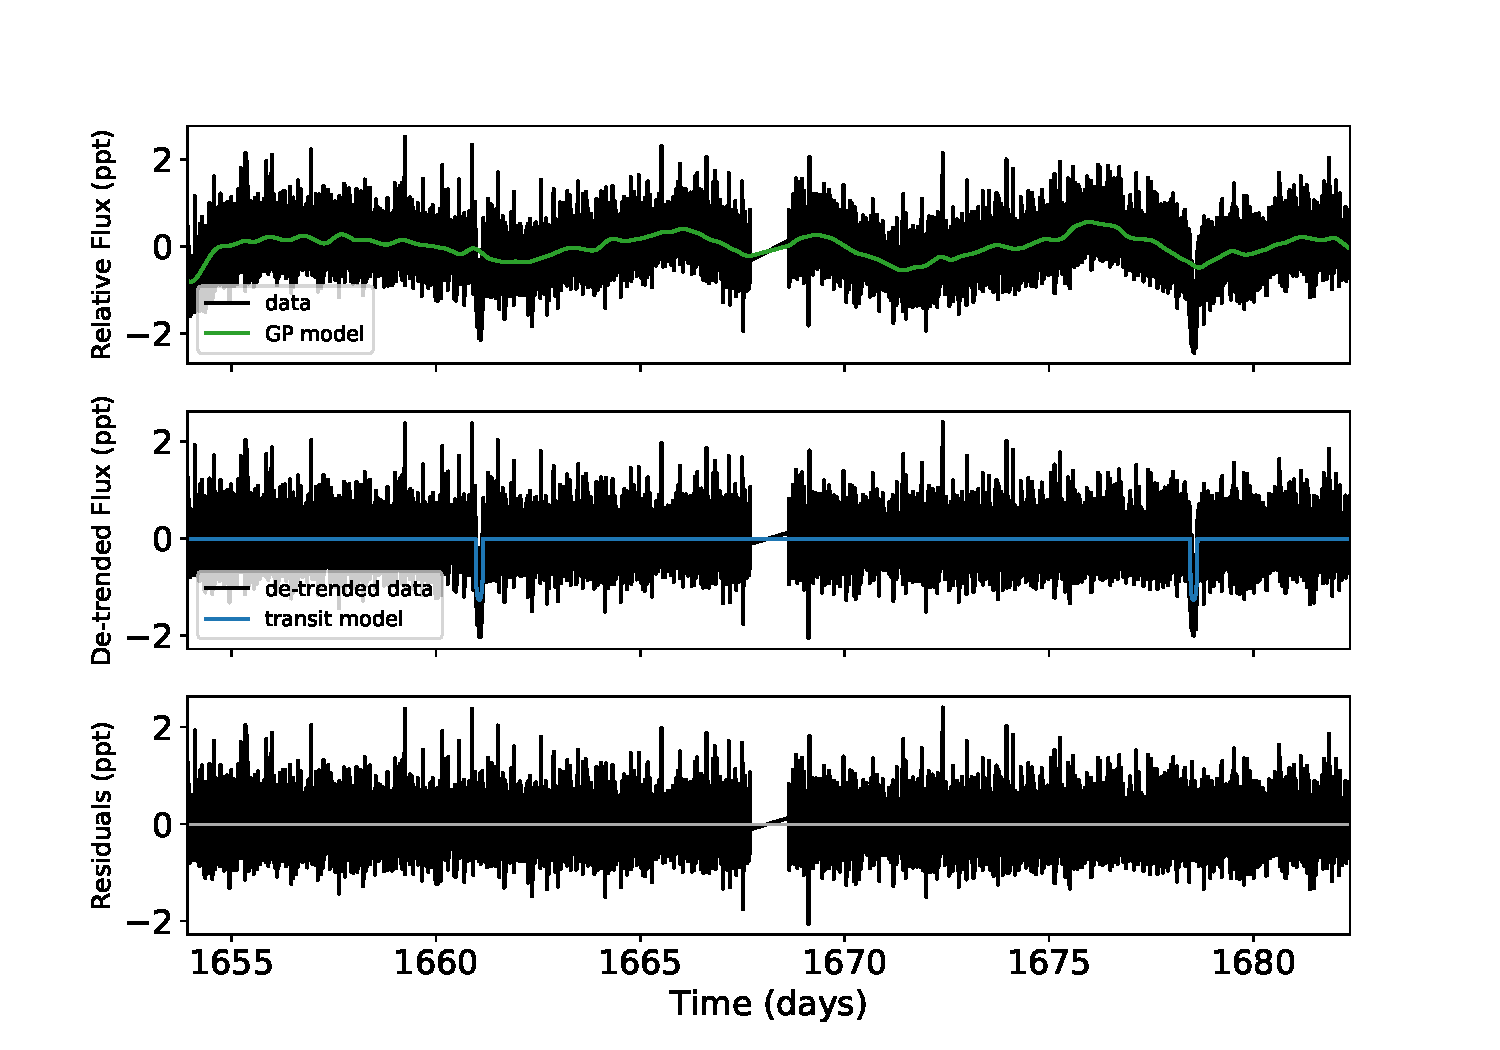
\includegraphics[width=\textwidth]{lightcurve.pdf}
    \caption{Photometric lightcurve of \hoststar as observed by \TESS in Sector 13. The \TESS data were fit with a Gaussian Process model (top panel) as a means of detrending. A transit model was simultaneously fit (middle panel), leaving a featureless white-noise lightcurve in the residuals (bottom panel).}
    \label{fig:lightcurve}
\end{figure}

\subsection{\RV-Only Analysis}
\label{s:analysis:rvs}

Although the orbital period and ephemerides of the planet candidate can be determined from the photometry, it can be informative to look for an independent signature of the planet's periodicity in the \RVs. 
In this particular case, we might have expected a 17-day super-Earth-sized planet to be detectable in the existing \RV time series, so testing this hypothesis by attempting to blindly recover the planet is a useful exercise in understanding any biases that might be present in the existing data analysis framework for the Solar Twin Planet Search \RV survey.

The first and simplest way to look for periodicity in the \RV data is with a Lomb-Scargle periodogram. 
One instrumental effect must be accounted for here. 
In June 2015, the \HARPS\ optical fibers were replaced as part of a major instrument upgrade, leaving an effective offset between \RVs and other line profile-sensitive components measured before and after the upgrade \citep{Lovis15}. 
For this initial inspection, we simply subtract an offset of 15.4 \ms from the post-upgrade \RVs. 
This quantity was derived from the median behavior of a set of \RV-quiet solar twins \citep{Melendez17}. 
The Lomb-Scargle periodogram of the offset-corrected \RVs does not show an obvious planet signal; instead, a forest of peaks is present around the 20-30 day expected rotation period, with significant strength at long periods as well. 
If stellar activity signals are present in the data, from surface features rotating across the star or from longer-term variations in the net convective blueshift suppression, they could complicate the periodogram in this way. 
In particular, the phase incoherence of activity signals due to constantly-evolving surface features over the long duration of \RV observations will lead to messy structures around the rotation period and its harmonics, which unfortunately coincide with the region of period space we wish to search. 
To deal with these issues, we require a slightly more advanced model than the pure sinusoid that is implicitly assumed in a Lomb-Scargle periodogram search.

A great many options exist for modeling stellar variability in \RVs, from autoregressive and Gaussian process (\GP) approaches to the use of simultaneous photometry (\todo{CITE}). 
Here, a simple and fast-to-compute model is desired, so despite the detailed inaccuracies of this assumption we adopted a linear relationship between \RV and an auxiliary activity indicator. 
We tested the correlation strength of \RVs against several activity indicators (\BIS, \FWHM, and \shk, as discussed in Section \ref{s:data:rvs}). 
Because the \HARPS\ optical fiber upgrade affected the line spread function of the instrument, offsets are present in the \BIS and \FWHM measurements. 
We dealt with these as in the \RVs by subtracting an offset of 0.01 fit by eye from the post-upgrade \BIS and \FWHM measurements. 
The results indicate a significant linear correlation between \RV and \FWHM in the data, with a Pearson correlation coefficient of \todo{0.7} and a bootstrapped false alarm probability of \todo{0.001}. 
Neither of the other activity indicators show strong correlations. 
We therefore adopt a linear \RV-\FWHM relationship in our model. 
We also add in a quadratic trend component to account for long-term changes in the \RVs due to either the evolving magnetic activity cycle or undetected long-period companions.

With this more advanced model, we constructed a \textit{log-likelihood periodogram}. 
This approach is a simple and efficient way of searching frequency space while taking certain systematic noise sources into account, and follows the methodology behind the Systematics-Insensitive Periodogram introduced for \kepler transit searches by \citet{Angus2016}. 
Specifically, in our application the model prediction is that for any time $t_n$ with corresponding \FWHM measurement $w_n$, the \RV $y_n$ is given by:
\begin{equation}
    y_n = a x_n^2 + b x_n + c_n + d w_n + K sin\Big(\frac{2\pi}{P} t_n\Big) + H cos\Big(\frac{2\pi}{P} t_n\Big) + \mathrm{noise},
\end{equation}
where $x_n$ is a normalized relative time:
\begin{equation}
    x_n = \frac{t_n - \langle t \rangle}{\mathrm{max}(t) - \mathrm{min}(t)},
\end{equation}
the baseline term $c_n$ is comprised of two possible values based on whether observation $n$ was taken before or after \HARPS upgrade time $t_{upgrade}$:
\begin{equation}
    c_n = \left\{
        \begin{array}{ll}
            c_1 & \quad t_n < t_{upgrade} \\
            c_2 & \quad t_n \geq t_{upgrade}
        \end{array}
    \right,
\end{equation}
and all other variables ($a, b, c_1, c_2, d, K, H, P$) are unknowns to be constrained from the data. 
At any given value of the orbital period $P$, this model is entirely linear, so that the vector of predicted \RVs $\mathbf{y}$ can be calculated as a product of variable vector
\begin{equation}
    \theta = [a, b, c_1, c_2, d, K, H]^T
\end{equation}
and design matrix
\begin{equation}
    A_P = 
    \begin{pmatrix}
        x_0^2 & x_0 & c_0 & w_0 &  sin\Big(\frac{2\pi}{P} t_n\Big) &  cos\Big(\frac{2\pi}{P} t_n\Big)\\
        \vdots & \vdots & \vdots\\
        x_n^2 & x_n & c_n
    \end{pmatrix}.
\end{equation}
At period $P$, then, the optimal parameters $\mathbf{\theta^*_P}$ can be analytically determined as the following:
\begin{equation}
    \mathbf{\theta^*_P} = .
\end{equation}
We step through a log-uniform grid of periods between 1 and 1000 days and determine the maximum likelihood for that period:
\begin{equation}
    log\mathcal{L}^*_P = .
\end{equation}
The resulting log-likelihood periodogram shares the fundamental assumption of a circular orbit but is otherwise more robust to stellar activity and long-period trends than the Lomb-Scargle approach. 
Due to the linearity of the model and the resulting ability to find the optimal parameters analytically, the likelihood may be maximized quickly and with a guarantee of convexity. 
Therefore, while more advanced tools exist to incorporate Bayesian priors \citep{Olspert2018} or non-parametric correlated noise \citep{Feng2017} along with trends in the data, this method is relatively simple to implement, flexible, and fast.

The log-likelihood periodogram does show a strong peak at 17 days (Figure \ref{fig:lnlikeperiodogram}). 
While this supports the presence of a sinusoidal, potentially Keplerian signal in the data, we note that this conclusion depends on the noise model adopted. 
The 17-day peak is the highest in the log-likelihood periodogram, but a forest of other strong peaks remain; these may arise from noise that was not accounted for in our model or from additional planets in the system. 

In brief, the above analysis shows that the \RV data do support the detection of a 17-day planet, but the signal is not sufficiently strong or robust to changes in the noise model to confidently claim detection on the grounds of \RVs alone.



\begin{figure}
    \centering
    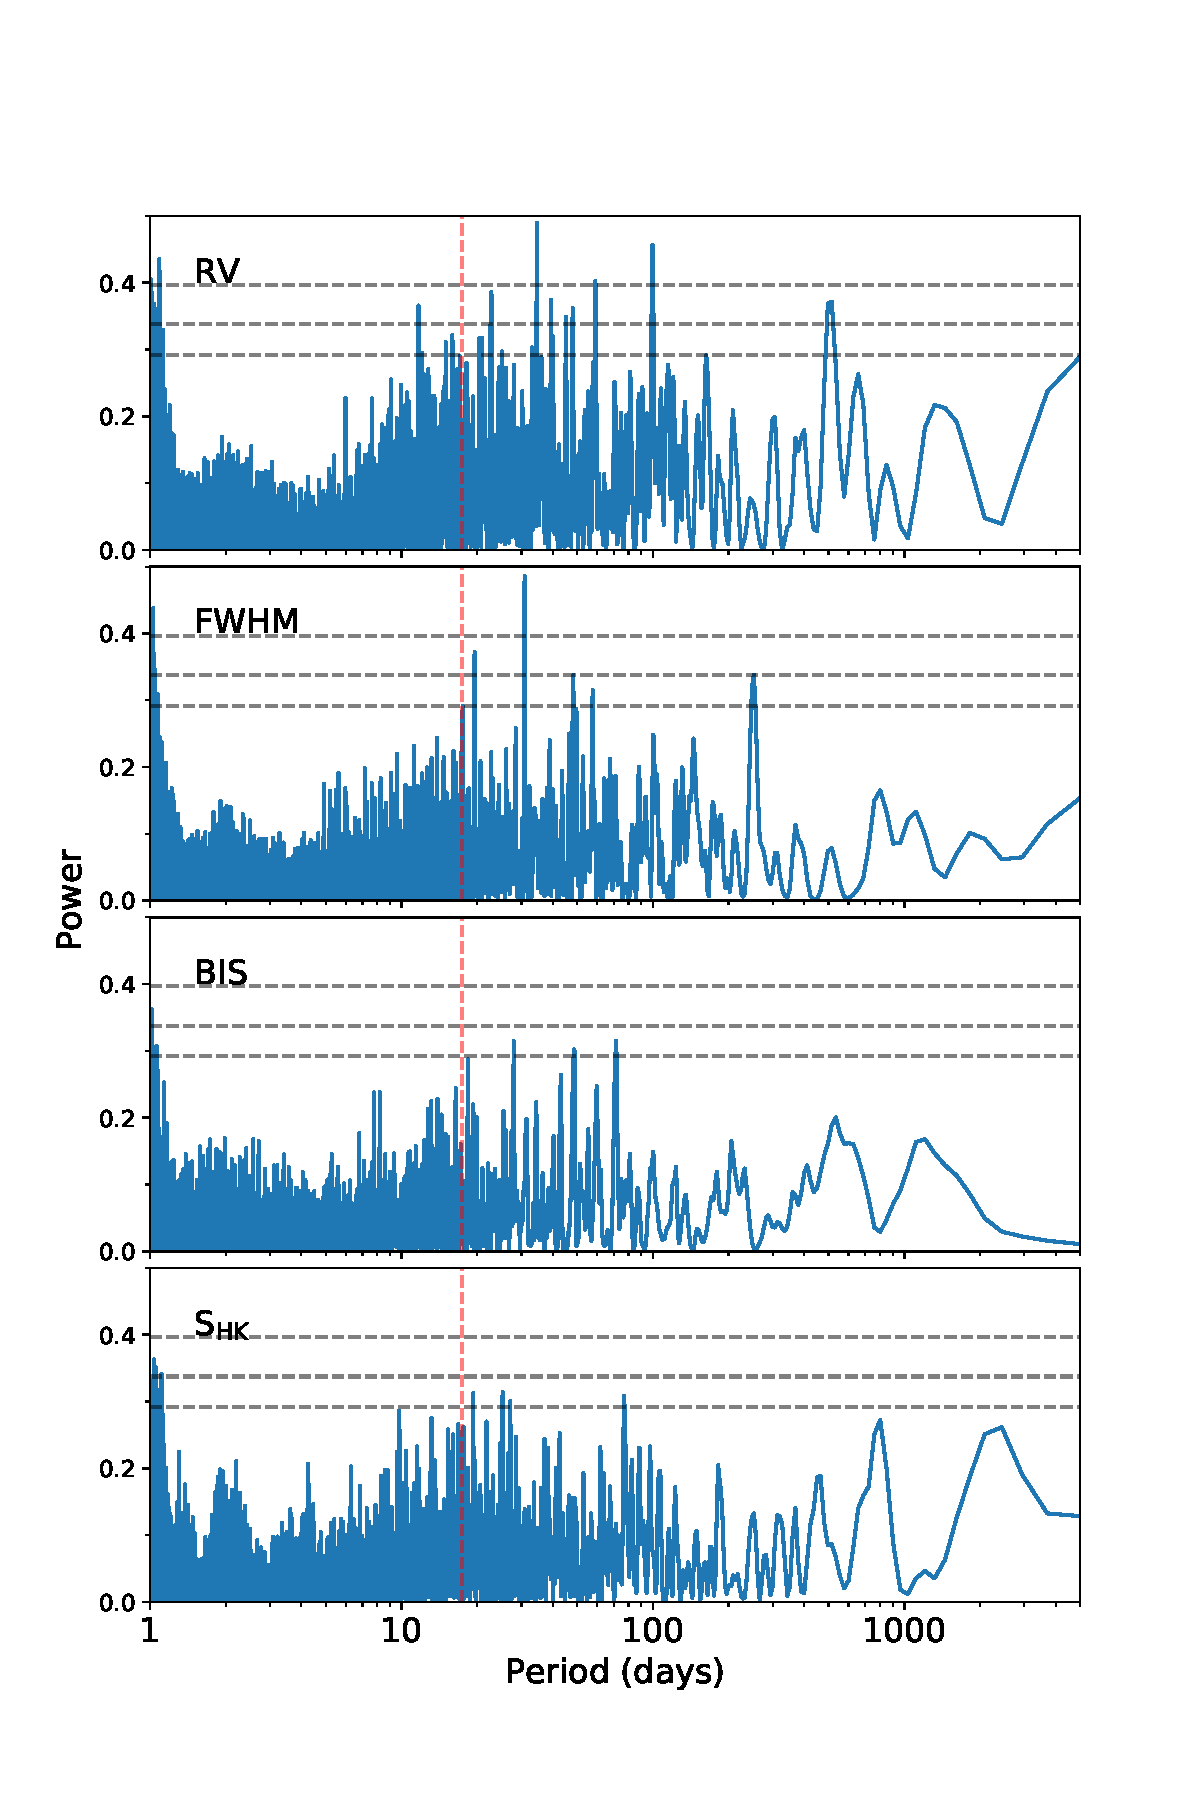
\includegraphics[width=\textwidth]{periodograms.pdf}
    \caption{Lomb-Scargle periodograms of the \HARPS\ \RV, BIS, FWHM, and \shk timeseries measurements. Horizontal lines indicate the 5\%, 1\%, and 0.1\% false alarm probability levels. Vertical red lines mark the period of the \TESS-detected planet. The \RV, BIS, and FWHM measurements used here have been corrected for the \HARPS upgrade offset.}
    \label{fig:periodograms}
\end{figure}


\subsection{Joint Analysis}
\label{s:analysis:joint}

\begin{figure}
    \centering
    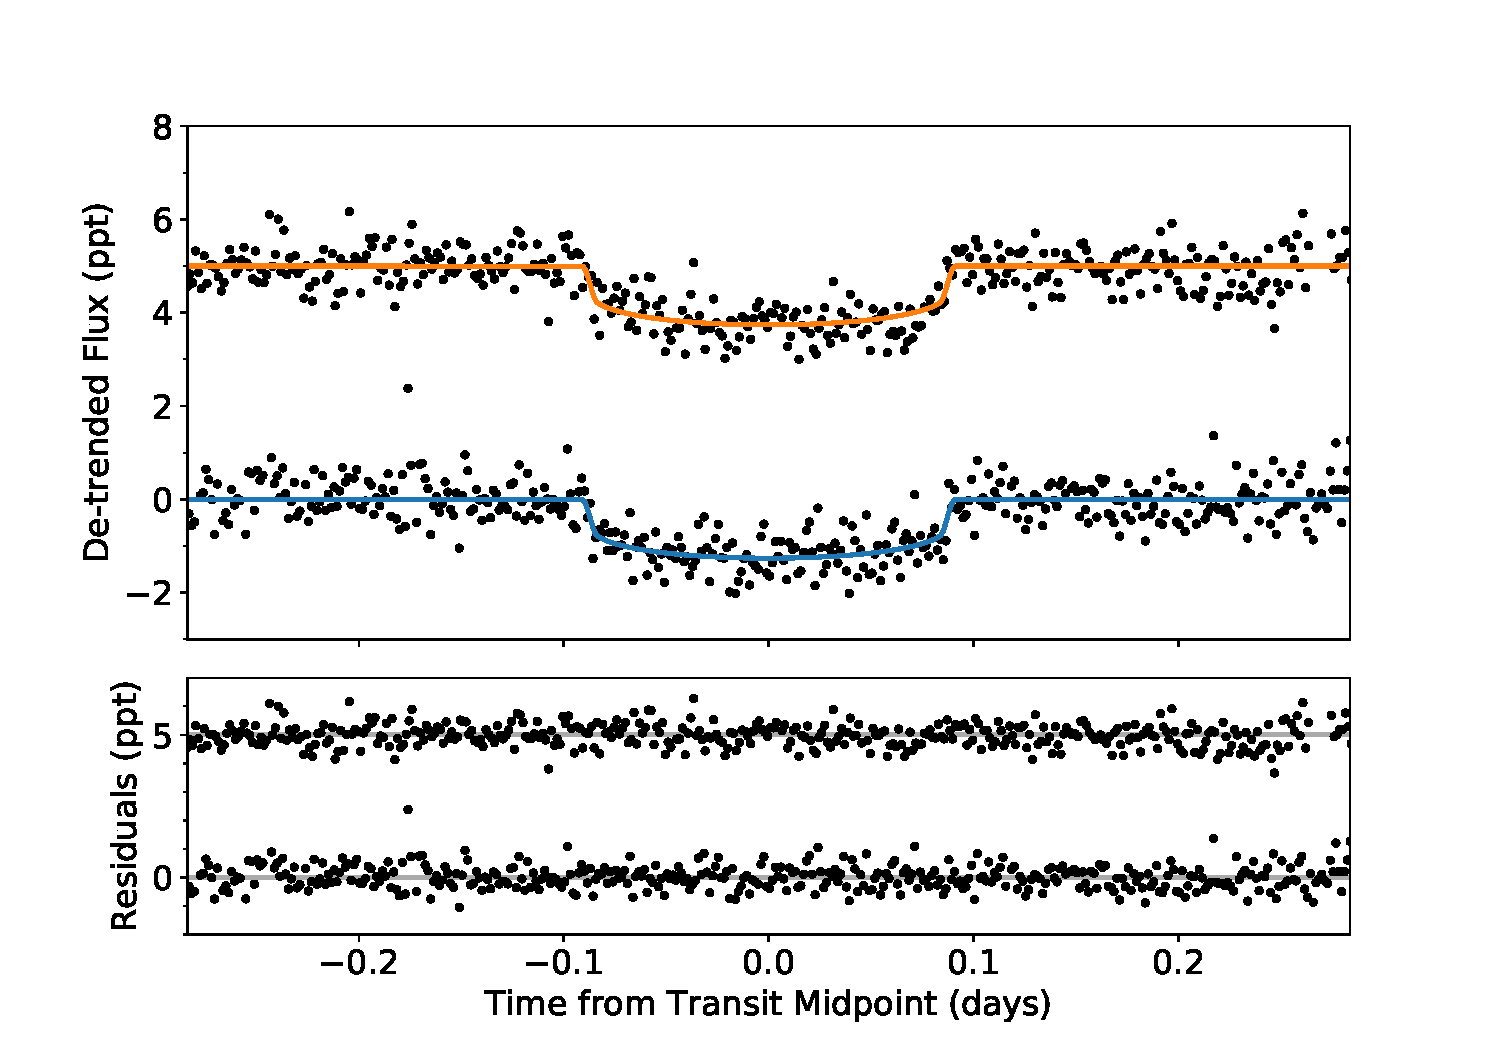
\includegraphics[width=\textwidth]{transits.pdf}
    \caption{De-trended lightcurve data and best-fit model for the two transit events in \TESS. Arbitrary offsets on the vertical axis were given to the separate events for clarity.}
    \label{fig:transits}
\end{figure}

\begin{figure}
    \centering
    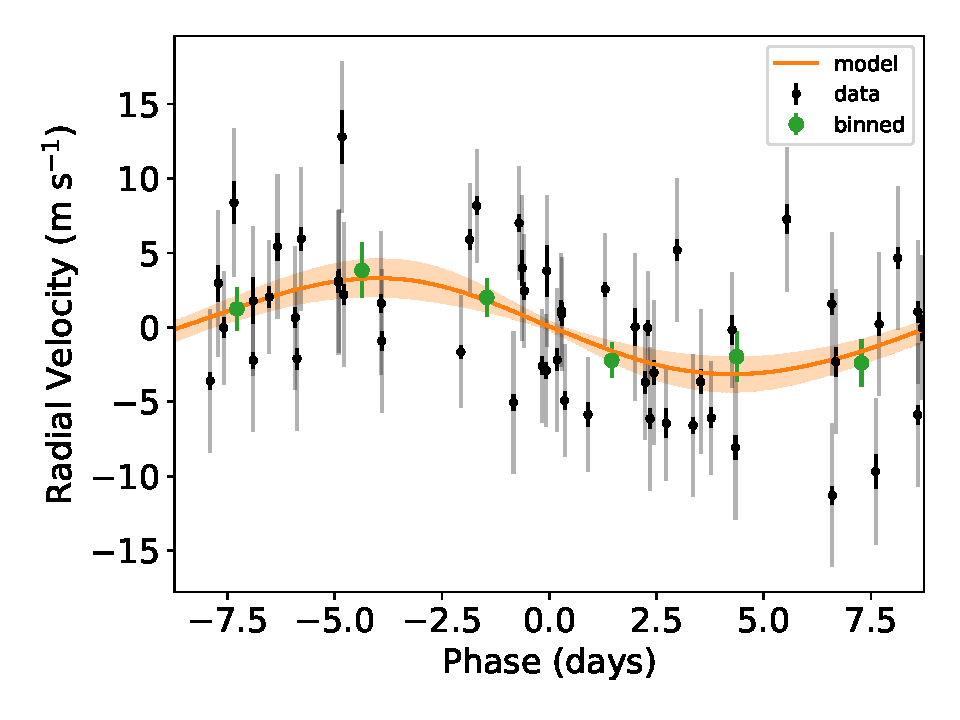
\includegraphics[width=16cm]{rvphased_1pl_wfwhm}
    \caption{Phase-folded radial velocities for \plname. Individual data points and their photon-noise-based uncertainties are shown as black points and error bars, while the grey error bars represent the uncertainties inflated by the best-fit (posterior median) jitter parameters. Green points are the error-weighted means within a series of phase bins. The best-fit model is shown as a solid orange line, with the shaded region around it marking the model's 1-$\sigma$ credible interval.}
    \label{fig:rv_phased}
\end{figure}


\section{Discussion}
\label{s:discussion}


(Low probability of background contaminants - discuss Gaia, spectra)

(reliability of the RV fit - potential for more planets? activity?)

(M-R diagram)

(prospects for further compositional analysis)

(prospects for atmospheric characterization)

(star \& Sun are very similar but ended up with very different planetary systems. why? bring up [lack of] giant planet companions, cite Bryan; if migration happened, it left no trace on the star. also cite Kepler-11 as another similar star to the Sun with a different planetary system architecture.)

\section{Conclusion}
\label{s:conclusion}


\acknowledgements
We thank Trevor David, ... for useful discussions.
This work is based on observations collected at the European Southern Observatory under ESO programmes 188.C-0265 and 0100.D-0444. 
This work has made use of data from the European Space Agency (ESA) mission
{\it Gaia} (\url{https://www.cosmos.esa.int/gaia}), processed by the {\it Gaia}
Data Processing and Analysis Consortium (DPAC,
\url{https://www.cosmos.esa.int/web/gaia/dpac/consortium}). Funding for the DPAC
has been provided by national institutions, in particular the institutions
participating in the {\it Gaia} Multilateral Agreement.

\software{
    \code{Astropy} \citep{astropy},
    \code{exoplanet} \citep{exoplanet},
    \code{IPython} \citep{ipython},
    \code{matplotlib} \citep{matplotlib},
    \code{numpy} \citep{numpy},
    \code{scipy} (\url{https://www.scipy.org/}),
}

\facility{TESS, HARPS}

\bibliographystyle{aasjournal}
\bibliography{ms}

\end{document}